%%%%%%%%%%%%%%%%%%%%%%%%%%%%%%%%%%%%%%%%%%%%%%%%%%%%%%%%%%%%%%%%%%%%%%%%%%%%%%%%
%2345678901234567890123456789012345678901234567890123456789012345678901234567890
%        1         2         3         4         5         6         7         8
%% PP_Report.tex
%% V2.1
%% 2017/05/07
%% by Rui Santos Cruz
%% This is a skeleton file using PPIEEEtran.cls
%% (requires PPIEEEtran.cls)
% !TEX root = ./main.tex
%%%%%%%%%%%%%%%%%%%%%%%%%%%%%%%%%%%%%%%%%%%%%%%%%%%%%%%%%%%%%%%%%%%%%%%%%%%%%%%%
\documentclass[a4paper,12pt,journal,twoside,compsoc]{PPIEEEtran}
\usepackage{hyperref}

% In the ReportType command chose "act" for Activity Report or "learn" for Learnings Report
\newcommand*{\ReportType}{}
% -----------------------------------------------------------------------------
% The Preamble document contains all the necessary Packages for typesetting
% Modify it to suit your needs
% -----------------------------------------------------------------------------
%%%%%%%%%%%%%%%%%%%%%%%%%%%%%%%%%%%%%%%%%%%%%%%%%%%%%%%%%%%%%%%%%%%%%%%%%%%%%%%%
%2345678901234567890123456789012345678901234567890123456789012345678901234567890
%        1         2         3         4         5         6         7         8
% Required Packages and commands
% --> Please Choose the MAIN LANGUAGE for the document in package BABEL (below)
% --> Please Choose the TYPE OF REPORT for the document in \ReportType (below)
% !TEX root = ./main.tex
% PP_Report_Preamble.tex
% V2.1
% 2017/05/07
% by Rui Santos Cruz
%%%%%%%%%%%%%%%%%%%%%%%%%%%%%%%%%%%%%%%%%%%%%%%%%%%%%%%%%%%%%%%%%%%%%%%%%%%%%%%%
%
% *** INPUT LANGUAGE PACKAGES ***
% Choose the main language in package Babel
\usepackage[main=english,portuguese]{babel}
\usepackage[utf8]{inputenc}
\usepackage{iflang}

\usepackage[margin={2cm, 2cm}]{geometry}
\setlength{\columnsep}{1cm}

% *** ACRONYM PACKAGES ***
% Put definition of Acronyms at the end of the document
\usepackage[printonlyused,nolist]{acronym}

% *** CITATION PACKAGES ***
\usepackage{cite}

% *** GRAPHICS RELATED PACKAGES ***
\usepackage[pdftex]{graphicx}
\DeclareGraphicsExtensions{.pdf,.jpeg,.png}

% *** MATH PACKAGES ***
\usepackage[cmex10]{amsmath}

% *** SPECIALIZED LIST PACKAGES ***
\usepackage{algorithmic}

% *** ALIGNMENT PACKAGES ***
\usepackage{array}

% *** SUBFIGURE PACKAGES ***
\usepackage[font=normalsize,labelfont=sf,textfont=sf]{subfig}
\captionsetup[table]{skip=10pt}

% *** FLOAT PACKAGES ***
\begingroup\expandafter\expandafter\expandafter\endgroup
\expandafter\ifx\csname IncludeInRelease\endcsname\relax
  \usepackage{fixltx2e}
\fi

% *** PDF, URL AND HYPERLINK PACKAGES ***
\usepackage{url}

% *** BACKGROUND Material ***
\usepackage{eso-pic}
\usepackage[
  contents={},
  opacity=1,
  scale=1,
  color=blue!90
  ]{background}

% *** CONDITIONALS ***
\usepackage{ifthen}

% Clever Referencing
% Note: portuguese is supported through "brazilian" option
\usepackage[\IfLanguageName{english}{english}{brazilian}]{cleveref}

% Custom Packages
\usepackage{amsmath}
\usepackage{graphicx}
\usepackage{xcolor}
\definecolor{light-gray}{gray}{0.9}
\usepackage{tikz}
\usepackage{float}
\usetikzlibrary{positioning,shapes,shadows,arrows}
\tikzstyle{abstract}=[rectangle, draw=black, rounded corners, fill=blue!40, drop shadow,
        text centered, anchor=north, text=white, text width=2.5cm, node distance= 1cm and 0.3cm]
\tikzstyle{comment}=[rectangle, draw=black, rounded corners, fill=green, drop shadow,
        text centered, anchor=north, text=white, text width=2cm]
\tikzstyle{myarrow}=[->, >=open triangle 90, thick]
\tikzstyle{line}=[-, thick]

\usepackage{hyperref}

\usepackage{listings}
\lstset{basicstyle=\ttfamily,
  showstringspaces=false,
  commentstyle=\color{red},
  keywordstyle=\color{blue}
}
\usepackage{booktabs}
%%%%%%%%%%%%%%%%%%%%%%%%%%%%%%%%%%%%%%%%%%%%%%%%%%%%%%%%%%%%%%%%%%%%%%%%%%%%%%%%

% correct bad hyphenation here
\hyphenation{op-tical net-works semi-conduc-tor}
%%%%%%%%%%%%%%%%%%%%%%%%%%%%%%%%%%%%%%%%%%%%%%%%%%%%%%%%%%%%%%%%%%%%%%%%%%%%%%%%
%2345678901234567890123456789012345678901234567890123456789012345678901234567890
%        1         2         3         4         5         6         7         8
\begin{document}

%%%%%%%%%%%%%%%%%%%%%%%%%%%%%%%%%%%%%%%%%%%%%%%%%%%%%%%%%%%%%%%%%%%%%%%%%%%%%%%%
%2345678901234567890123456789012345678901234567890123456789012345678901234567890
%        1         2         3         4         5         6         7         8
%% PP_Report_Cover.tex
%% V2.1
%% 2017/05/07
%% by Rui Santos Cruz
% !TEX root = ./main.tex
%%%%%%%%%%%%%%%%%%%%%%%%%%%%%%%%%%%%%%%%%%%%%%%%%%%%%%%%%%%%%%%%%%%%%%%%%%%%%%%%
% paper title
% can use linebreaks \\ within to get better formatting as desired
% Do not put math or special symbols in the title.
\title{Raytracer}

%%%%%%%%%%%%%%%%%%%%%%%%%%%%%%%%%%%%%%%%%%%%%%%%%%%%%%%%%%%%%%%%%%%%%%%%%%%%%%%%
% Author names
%
% note positions of commas and nonbreaking spaces ( ~ ) LaTeX will not break
% a structure at a ~ so this keeps an author's name from being broken across
% two lines.
% use \thanks{} to gain access to the first footnote area
% a separate \thanks must be used for each paragraph.
%
%\IEEEcompsocitemizethanks is a special \thanks that produces the bulleted
% lists for "first footnote" author affiliations.
% Use \IEEEcompsocthanksitem which works much like \item
% for each affiliation group.
\author{Alexandre Gbaguidi Aïsse,
        Thibaud Michaud,
        Laurent Xu% <-this % stops a space
% Change the Course Name
% note: need leading \protect in front of \\ to get a newline within \thanks as
% \\ is fragile and will error, could use \hfil\break instead.
\IEEEcompsocitemizethanks{
\IEEEcompsocthanksitem Alexandre Gbaguidi Aïsse\protect\\
E-mail: aga@lrde.epita.fr,
\IEEEcompsocthanksitem Thibaud Michaud,\protect\\
E-mail: tmichaud@lrde.epita.fr
\IEEEcompsocthanksitem Laurent Xu,\protect\\
E-mail: lxu@lrde.epita.fr\protect\\
LRDE (Research and Development Laboratory of EPITA).\protect\\}% <-this % stops an unwanted space}% <-this % stops an unwanted space
\thanks{As part of the Image synthesis course at Epita.}
}
%%%%%%%%%%%%%%%%%%%%%%%%%%%%%%%%%%%%%%%%%%%%%%%%%%%%%%%%%%%%%%%%%%%%%%%%%%%%%%%%
% The paper headers
\markboth{Raytracer}%
% for a single student
%{Surname}% : for a single student
% for a Group Report
{Michaud \MakeLowercase{\textit{et al.}}}% : for a Group Report
%
% The only time the second header will appear is for the odd numbered pages
% after the title page when using the twoside option.

%%%%%%%%%%%%%%%%%%%%%%%%%%%%%%%%%%%%%%%%%%%%%%%%%%%%%%%%%%%%%%%%%%%%%%%%%%%%%%%%
% Prints in Subtitle the type of Report
% PLEASE DO NOT CHANGE THIS SECTION
%\IEEEspecialpapernotice{%
%\ifthenelse{\equal{\ReportType}{act}}{%
%\tlangRepActivity}{\tlangRepLearning}
%}
%%%%%%%%%%%%%%%%%%%%%%%%%%%%%%%%%%%%%%%%%%%%%%%%%%%%%%%%%%%%%%%%%%%%%%%%%%%%%%%%

%%%%%%%%%%%%%%%%%%%%%%%%%%%%%%%%%%%%%%%%%%%%%%%%%%%%%%%%%%%%%%%%%%%%%%%%%%%%%%%%
% The paper Abstract and Keywords
\IEEEtitleabstractindextext{%

\begin{abstract}
Today, Ray tracing is exclusively used for non real-time renderies because of
its slowness compare to rasterization techniques which dominate todays graphics
hardware. It is believed that ray tracing will not ever challenge rasterization
techniques. This report modestly contribute to this problem. We present our
implementation of an optimized C++11 raytracer and discuss about its
performances.
\end{abstract}
%
\begin{IEEEkeywords}
Raytracing, CUDA, real-time, rendering, GPU
\end{IEEEkeywords}}
%%%%%%%%%%%%%%%%%%%%%%%%%%%%%%%%%%%%%%%%%%%%%%%%%%%%%%%%%%%%%%%%%%%%%%%%%%%%%%%%

% make the title area
\maketitle

\IEEEdisplaynontitleabstractindextext
\IEEEpeerreviewmaketitle
%%%%%%%%%%%%%%%%%%%%%%%%%%%%%%%%%%%%%%%%%%%%%%%%%%%%%%%%%%%%%%%%%%%%%%%%%%%%%%%%
%%%%%%%%%%%%%%%%%%%%%%%%%%%%%%%%%%%%%%%%%%%%%%%%%%%%%%%%%%%%%%%%%%%%%%%%%%%%%%%%
\section{Introduction}
% The very first letter is a 2 line initial drop letter followed
% by the rest of the first word in caps (small caps for compsoc).
%
% form to use if the first word consists of a single letter:
% \IEEEPARstart{A}{demo} file is ....
%
% Here we have the typical use of a "E" for an initial drop letter
% and "STE" in caps to complete the first word.
\IEEEPARstart{I}{n} the context of computer graphics, \textit{rendering}~\cite{rendering} is the automatic process of generating an image from a 2D or a 3D model. Two major rendering categories exist: algorithms based on rasterization and those based on raytracing. Historically, raytracing has been used exclusively to produce high-quality images. This approach is well known for its poor performances and long rendering time. If more precision is needed then more time-consumption will occur because more rays will be casted.\\
\indent In this report, we present a raytracer with two modes: an interactive
real-time mode with a camera which can be used to walk around the scene and a
traditional mode that renders a single PPM image. We provide a command-line way
to enable and disable some features. For instance, you would like to disable
the refraction when using the interactive mode.\\
\indent After introducing in Section~\ref{spec} some specifications including
the input format, we detail our architecture in Section~\ref{impl}. From
Section~\ref{cam} to the end, we discuss about the implementation of
different part of the project.

%%%%%%%%%%%%%%%%%%%%%%%%%%%%%%%%%%%%%%%%%%%%%%%%%%%%%%%%%%%%%%%%%%%%%%%%%%%%%%%%
\section{Specifications}
\label{spec}
\IEEEPARstart{T}{his} section gives an overview of the project and explains different ways to use it.
\subsection{Description}
The main purpose of this project is to implement a raytracer with different
features. However, we also provide a real-time mode with the possibility to
enable or disable any features. This is quite interesting to realise the cost
of each method. Usually in raytracing, photo-realistic images are incompatible
with real-time rendering.
To summarize, from a given input which describes a scene, we give two possibilities:
\begin{itemize}
\item render the scene by producing an image and end the process.
\item enter in an interactive mode with a camera (point-of-view) that can be moved around the scene.
\end{itemize}

\subsection{Input}
The format of the input file is shown in~\ref{Fig:input}

The input file looks like this: \\
\begin{figure*}
\noindent\fcolorbox{blue}{light-gray}{%
    \minipage[t]{\dimexpr1\linewidth-2\fboxsep-2\fboxrule\relax}
    	screen width height \\
        camera pos$_x$ pos$_y$ pos$_z$ u$_x$ u$_y$ u$_z$ v$_x$ v$_y$ v$_z$ \\
        sphere radius pos$_x$ pos$_y$ pos$_z$ diff refl spec shin color$_r$ color$_g$ color$_b$ refr opac \\
    	plane a b c d diff refl spec shin color$_r$ color$_g$ color$_b$ refr opac \\
        triangle A$_x$ A$_y$ A$_z$ B$_x$ B$_y$ B$_z$ C$_x$ C$_y$ C$_z$ diff refl spec shin color$_r$ color$_g$ color$_b$ refr opac \\
        plight pos$_x$ pos$_y$ pos$_z$ color$_r$ color$_g$ color$_b$ \\
        dlight dir$_x$ dir$_y$ dir$_z$ color$_r$ color$_g$ color$_b$ \\
        alight color$_r$ color$_g$ color$_b$
    \endminipage}\vspace{0.3cm}
\caption{Input file format}
\label{Fig:input}
\end{figure*}
    where:
    \begin{itemize}
    	\small
    	\setlength{\itemsep}{0.2pt}
        \item camera has a position pos$_x$ pos$_y$ pos$_z$ and looks at the plane formed by the vectors (u$_x$, u$_y$, u$_z$) and (v$_x$, v$_y$, v$_z$).
        \item plane, triangle, sphere, etc. are the shapes that will be rendered
        \item (a-d-p)light is for ambiant, directional or point light
    	\item diff is the diffusion coefficient, between 0 and 1.
    	\item refl is the reflection coefficient, between 0 and 1.
        \item spec is the specular coefficient, between 0 and 1.
        \item shin is the shininess, between 0 and $\infty$. This property is used when implementing the specular light.
        \item color$_r$, color$_g$, color$_b$ contain three integer values, respectively the red, green and blue components, between 0 and 255.
		\item refr is the refraction coefficient, between 0 and $\infty$.
        \item opac is the opacity coefficient, between 0 and 1.
    \end{itemize}
For example, the input file of Figure~\ref{Fig:shadow} is the following:\\
\noindent\fcolorbox{blue}{light-gray}{%
    \minipage[t]{\dimexpr1\linewidth-2\fboxsep-2\fboxrule\relax}
    	screen 600 600 \\
        camera 0 0 0 1 0 0 0 1 0 \\
		sphere 2 -3 0 20 1 0 0 100 0 255 255 0 0 \\
		sphere 3 3 0 20 1 0 0 100 255 0 255 0 0 \\
		plane 0 1 0 -4 1 0 0 100 150 0 0 0 0 \\
		alight 255 255 255 \\
		dlight 1 1 0 255 255 255 \\
		dlight -1 1 0 255 255 255
    \endminipage}

\subsection{Output}
As said before, we offer two ways to use our raytracer: a basic image rendering and an interactive mode. The basic mode outputs a picture using the PPM~\cite{ppm} format. In the interactive mode, each time the camera moves, its new coordinates are taken into account and the scene is recomputed. The graphics and events are handled using the SFML~\cite{sfml} library. To move the camera, use the keyboard arrows.

\begin{figure}
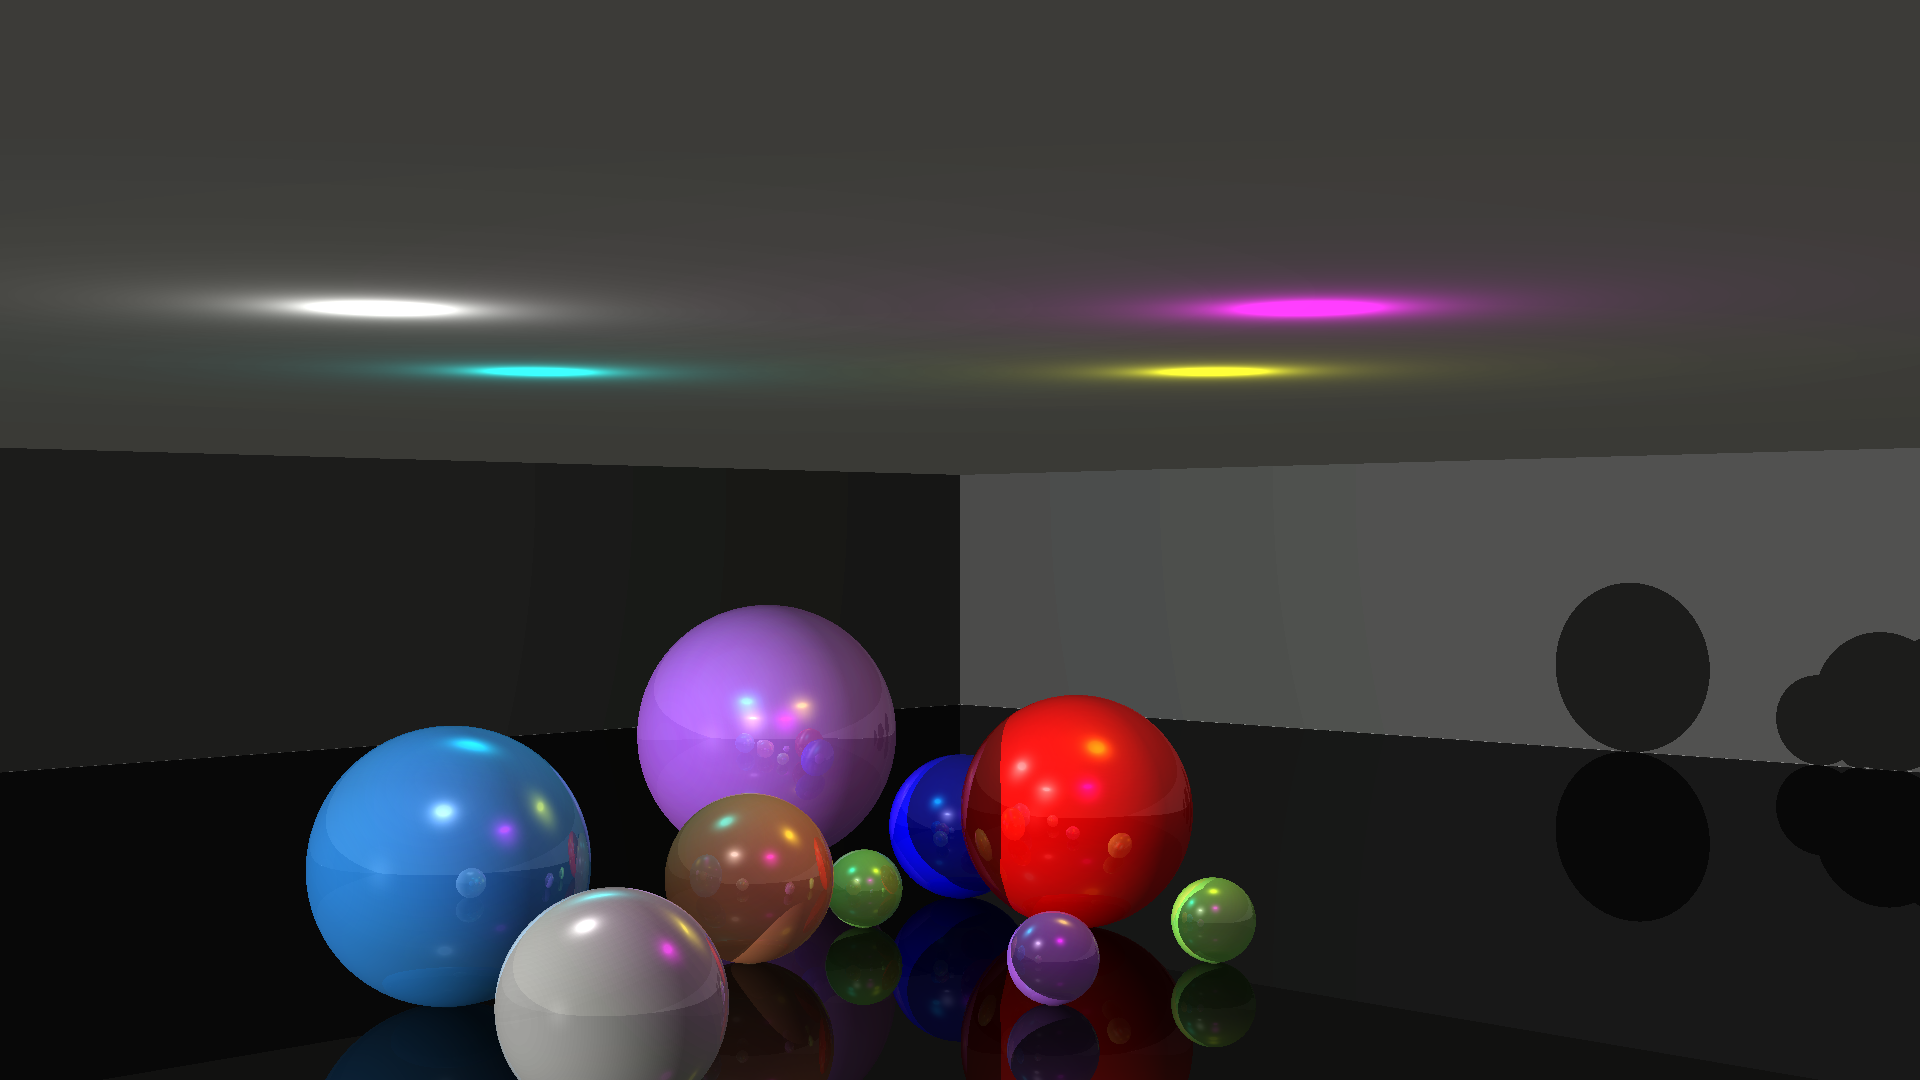
\includegraphics[width=\linewidth]{corner.png}
\caption{Example of a scene rendered with our raytracer to demonstrate ponctual
  lights, directional lights and shadows}
\label{Fig:shadow}
\end{figure}

%%%%%%%%%%%%%%%%%%%%%%%%%%%%%%%%%%%%%%%%%%%%%%%%%%%%%%%%%%%%%%%%%%%%%%%%%%%%%%%%
\section{Architecture}
\label{impl}

\IEEEPARstart{T}{he} Figure~\ref{Fig:raycast} shows the camera position and its field-of-view (fov).
Here are the steps\footnote{This part is heavily based on a subject written by the ACU 2016 of EPITA.} to compute outgoing screen vectors:
\begin{itemize}
\small
\item Normalize $u$ and $v$.
\item Compute $w$ using cross-product between $u$ and $v$.
\item Compute $L$, the distance between the eye and the center of the screen, according to $\tan(\textit{fov}) = \dfrac{\textit{screenwidth}}{2}$
\item Compute $C$, the center of the screen according to $C - Lw = eye\_pos$.
\item Now, from $\dfrac{-\textit{screenwidth}}{2}$ to $\dfrac{\textit{screenwidth}}{2}$ and from $\dfrac{-\textit{screenheight}}{2}$ to $\dfrac{\textit{screenheight}}{2}$ :
	\begin{itemize}
	\item Compute the point on the screen using $u$ and $v$.
    \item Using this point and the eye position, compute the outgoing vector.
    \item Using the position of the camera and the vector from the eye to the point on the screen, cast the ray.
	\end{itemize}
\end{itemize}

\begin{figure}
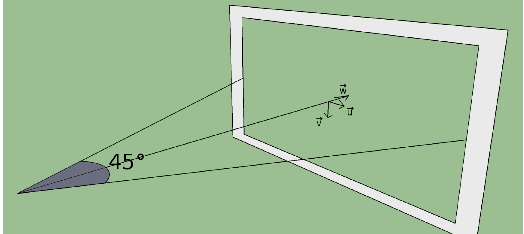
\includegraphics[scale=1]{two}
\caption{Raytracing concept}
\label{Fig:raycast}
\end{figure}

A class named data (Figure~\ref{Fig:umldata}) is instantiated at the beginning of
the program. Then the program parses the input file and fills the data. And since
Sphere, Plane and Triangle are some type of Object, those specific objects
inherit from a base class Object (Figure~\ref{Fig:umlobj}). Such an implementation
makes the rest of the code more generic. We did the same with lights
(Figure~\ref{Fig:umllight}).

\begin{figure}
\centering
\begin{tikzpicture}[node distance=2cm]
    \node (Object) [abstract, rectangle split, rectangle split parts=2]
        {
            \textbf{Object}
            \nodepart{second}intersect()
        };
    \node (Plane) [abstract, rectangle split, rectangle split parts=2, below=of Object]
        {
            \textbf{Plane}
            \nodepart{second}intersect()
        };
    \node (Sphere) [abstract, rectangle split, rectangle split parts=2, left=of Plane]
        {
            \textbf{Sphere}
            \nodepart{second}intersect()
        };
    \node (Triangle) [abstract, rectangle split, rectangle split parts=2, right=of Plane]
        {
            \textbf{Triangle}
            \nodepart{second}intersect()
        };
	\draw[myarrow] (Sphere.north) -- ++(0,0.5) -| (Object.south);
    \draw[line] (Plane.north) -- ++(0,0.6);
    \draw[line] (Sphere.north) -- ++(0,0.5) -| (Triangle.north);
\end{tikzpicture}
\caption{Base class Object and each kind of object that inherits from it.}
\label{Fig:umlobj}
\end{figure}

\begin{figure}
\centering
\begin{tikzpicture}[node distance=2cm]
    \node (Light) [abstract, rectangle split, rectangle split parts=2]
        {
            \textbf{Light}
            \nodepart{second}apply()\\in\_shadow()\\factor()
        };
    \node (Dlight) [abstract, rectangle split, rectangle split parts=2, below=of Light]
        {
            \textbf{Dlight}
            \nodepart{second}in\_shadow()\\factor()
        };
    \node (Alight) [abstract, rectangle split, rectangle split parts=2, left=of Dlight]
        {
            \textbf{Alight}
            \nodepart{second}in\_shadow()\\factor()
        };
    \node (Plight) [abstract, rectangle split, rectangle split parts=2, right=of Dlight]
        {
            \textbf{Plight}
            \nodepart{second}in\_shadow()\\factor()
        };
	\draw[myarrow] (Alight.north) -- ++(0,0.5) -| (Light.south);
    \draw[line] (Dlight.north) -- ++(0,0.6);
    \draw[line] (Alight.north) -- ++(0,0.5) -| (Plight.north);
\end{tikzpicture}
\caption{Base class Light and each kind of light that inherits from it.}
\label{Fig:umllight}
\end{figure}

\begin{figure}
\centering
\begin{tikzpicture}[node distance=2cm]
    \node (Data) [abstract, rectangle split, rectangle split parts=2]
        {
            \textbf{Data}
            \nodepart{second}width\\height\\vector Object\\%
            vector Light
        };
\end{tikzpicture}
\caption{Data class}
\label{Fig:umldata}
\end{figure}

\section{Camera}
\label{cam}
In this section we describe how the right vector, the up vector and the
position of the camera are updated using the arrow keys of the keyboard and the
mouse position.

\subsection{Translation}

The arrow keys of the keyboard allow the user to translate the camera following
the right vector or the front vector. Since we, already have the right vector
the method is trivial for the left and right arrows, we just need to add to the
position of the camera the right vector. For the up and down arrow we need to
define the front vector. This can easily be defined using a cross product between
the up vector and the right vector.

\subsection{Rotation}

The idea of the rotation is to find the right values of the right and up vectors
using the pitch roll and yaw roll. At each frame we compute the variation
of position of the mouse. This variation on the x-axis will affect the yaw
roll. While the variation on the y-axis will affect the pitch roll. Then
we compute the right and the up vectors as follows, where init\_up is the
initial value of the up vector:
\begin{align*}
  \text{front.x} := cos(\text{yaw}) * cos(\text{pitch}) \\
  \text{front.y} := sin(\text{pitch}) \\
  \text{front.z} := sin(\text{yaw}) * cos(\text{pitch}) \\
  \text{front} := normalize(\text{front}) \\
  \text{right} := \text{front} \times \text{init\_up} \\
  \text{up} := \text{right} \times \text{front} \\
\end{align*}

%%%%%%%%%%%%%%%%%%%%%%%%%%%%%%%%%%%%%%%%%%%%%%%%%%%%%%%%%%%%%%%%%%%%%%%%%%%%%%%%
\section{Camera}

%%%%%%%%%%%%%%%%%%%%%%%%%%%%%%%%%%%%%%%%%%%%%%%%%%%%%%%%%%%%%%%%%%%%%%%%%%%%%%%%
\section{Shadows}

%%%%%%%%%%%%%%%%%%%%%%%%%%%%%%%%%%%%%%%%%%%%%%%%%%%%%%%%%%%%%%%%%%%%%%%%%%%%%%%%
\section{Refraction}

Refraction is the phenomenon deviating rays of lights when they enter
transparent objects.  The angle of this deviation is ruled by an equation
summarized in \cref{fig:refr}, where $n_1$ is the refractive index of the medium
from which the light comes, and $n_2$ is that of the medium in which it enters.
\begin{figure}
  \begin{center}
    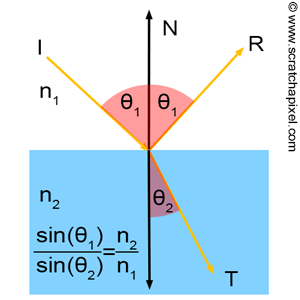
\includegraphics[width=0.7\linewidth]{refraction.png}
  \end{center}
  \caption{Refraction law}
  \label{fig:refr}
\end{figure}

With some trigonometry, we can compute the angle of this refracted ray.  Since
some objects are both reflective and refractive, we must throw 2 rays at each
collision.  For this, we recursively call our \texttt{cast} method twice, once
for the reflected ray and once for the refracted ray, and multiply the results
of these casts by the coefficients indicated in the configuration file for the
object corresponding to the collision.

A sample image with refractive spheres is shown in \cref{fig:sample-refr}.  The
refractive index of the spheres is that of glass (1.53).

\begin{figure*}
  \begin{center}
    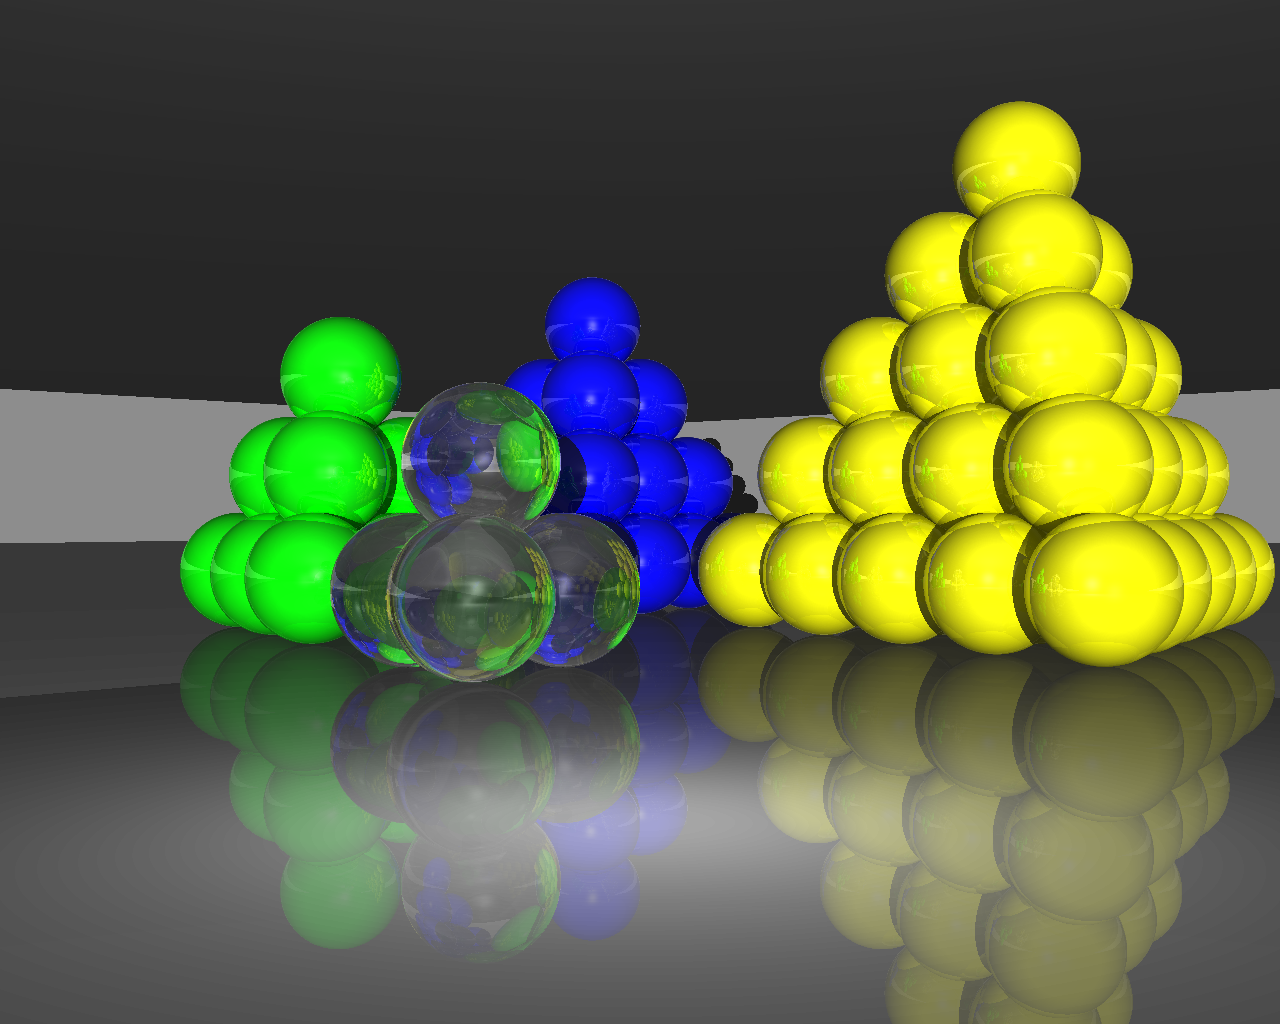
\includegraphics[width=0.7\linewidth]{sample-refraction.png}
  \end{center}
  \caption{Refractive spheres}
  \label{fig:sample-refr}
\end{figure*}

%%%%%%%%%%%%%%%%%%%%%%%%%%%%%%%%%%%%%%%%%%%%%%%%%%%%%%%%%%%%%%%%%%%%%%%%%%%%%%%%
\section{Perlin}

Perlin noise is the most common technique for generating random but coherent
patterns.  It is based on the computation of random gradients on the vertices of
an n dimensional grid, and the values at each point in the continuous space is
computed based on an interpolation of these gradients.  The closer a point is
from a vertice of the grid, the higher the contribution of the corresponding
gradient to the final value assigned to this point.  The computed value can be
used in several ways.  We can use it to generate random patterns of colors as a
texture for the objects, as in \cref{fig:perlin-color}.  This picture also
demonstrates the effect of modifying the frequency of the perlin noise: a higher
frequency generates smaller patterns.  Another way we can use the perlin noise
is to randomize the normal of collisions, thus affecting the way the the object
is rendered at this point as shown in \cref{fig:perlin-normal}.

\begin{figure*}
  \begin{center}
    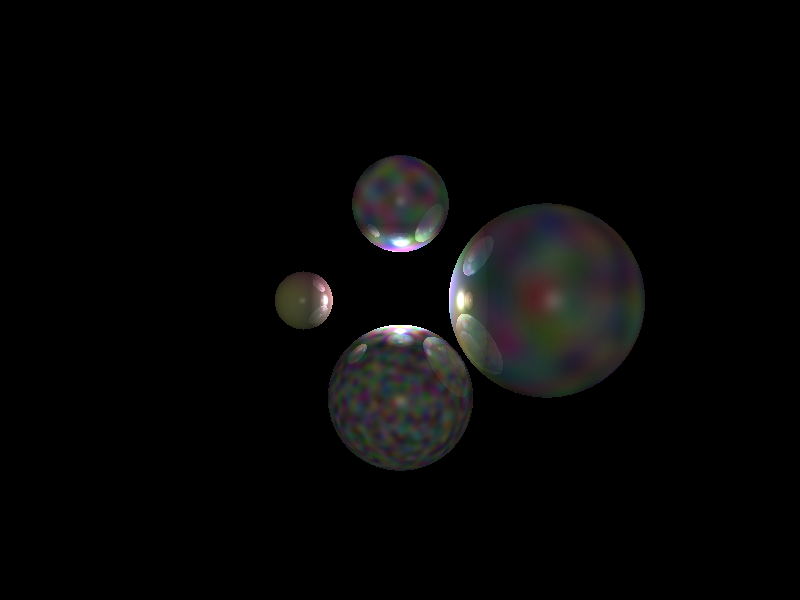
\includegraphics[width=0.7\linewidth]{perlin-color.png}
  \end{center}
  \caption{Perlin noise on object's color with various frequencies.}
  \label{fig:perlin-color}
\end{figure*}

\begin{figure*}
  \begin{center}
    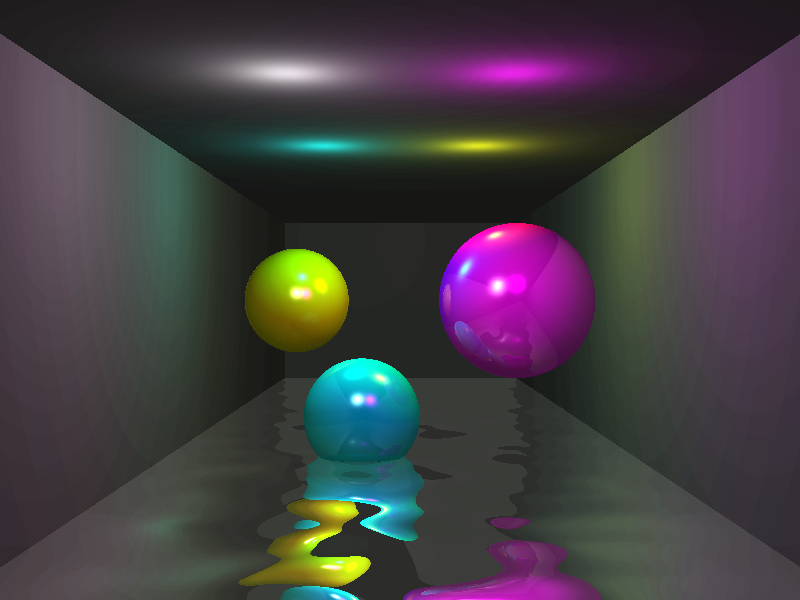
\includegraphics[width=0.7\linewidth]{perlin-normal.png}
  \end{center}
  \caption{Perlin noise on a plane's normal.}
  \label{fig:perlin-normal}
\end{figure*}

%%%%%%%%%%%%%%%%%%%%%%%%%%%%%%%%%%%%%%%%%%%%%%%%%%%%%%%%%%%%%%%%%%%%%%%%%%%%%%%%
\section{Difficulties encountered}

%%%%%%%%%%%%%%%%%%%%%%%%%%%%%%%%%%%%%%%%%%%%%%%%%%%%%%%%%%%%%%%%%%%%%%%%%%%%%%%%
\section{Conclusion}
\label{concl}
\IEEEPARstart{A}{} C++ implementation of a raytracer has been presented. This
raytracer contains several features such as refraction and perlin that can
easily be enabled or disabled. We proposed two ways to use our raytracer: an
interactve mode with a moving camera and a usual mode that outputs a single
PPM image.

%%%%%%%%%%%%%%%%%%%%%%%%%%%%%%%%%%%%%%%%%%%%%%%%%%%%%%%%%%%%%%%%%%%%%%%%%%%%%%%%

% references section
\bibliographystyle{IEEEtran}
\bibliography{bib}
%%%%%%%%%%%%%%%%%%%%%%%%%%%%%%%%%%%%%%%%%%%%%%%%%%%%%%%%%%%%%%%%%%%%%%%%%%%%%%%%
\newpage
\onecolumn

\end{document}
